
\chapter{Protección contra contactos directos e indirectos}

El paso de la corriente eléctrica por el cuerpo humano puede llevar a lesiones que van desde quemaduras leves hasta la muerte.

La descarga puede ocurrir al producirse un \textbf{contacto directo} del cuerpo con alguna parte de la instalación, o bien a través de un \textbf{contacto indirecto} con alguna de las masas puestas accidentalmente en tensión.

\begin{ejemplo}
	Un niño que toque la parte metálica del terminal fase de un interruptor, recibirá una descarga eléctrica por encontrarse en \textbf{contacto directo} con una de las partes vivas de la instalación.
	
	Al ocurrir una falla en una heladera, toda su carcaza metálica queda en contacto con el conductor fase. Cuando una persona toque esta carcaza, recibirá una descarga por \textbf{contacto indirecto}.
\end{ejemplo}

Existen distintos \textbf{esquemas de conexión a tierra} que permiten proteger a las personas y animales ante contactos directos e indirectos.

En Argentina, rige la norma 90364 de la Asociación Electrotécnica Argentina, basado en la Norma IEC 60364. Dicha norma, fue la que se tomó como base para escribir este documento.

Lo que se pretende en el reglamento es proteger a las personas, a las instalaciones contra los incendios de origen eléctrico, proteger de sobrecargas y cortocircuitos, proteger a los materiales y a los equipos contra sobretensiones y a las personas y animales de contactos directos e indirectos.

\section{Dispositivos de protección}
\textbf{Fusible}

Consiste en un conductor de diámetro menor al del resto de la instalación. Ante un eventual cortocircuito, el exceso de corriente provocará que el fino conductor se funda, protegiendo al resto de la instalación. El fusible se utiliza sólo una vez. Es decir que cuando su filamento se funde, debe ser modificado.

\textbf{Interruptor termomagnético}

Se trata de un dispositivo que consiste en un electroimán y un sensor bimetálico conectados en serie.

Al producirse un exceso de corriente, la temperatura aumenta en el bimetal, y éste, que funciona como un interruptor normalmente cerrado, se abre e interrumpe el circuito. También es posible que la corriente active el electroimán, y que éste actúe mecánicamente abriendo el circuito. Finalmente, se cuenta con una llave manual para activar y desactivar el interruptor.

\textbf{Interruptor diferencial}

Se trata de un interruptor que sensa, a través de una bobina toroidal, la corriente de entrada y de salida de la instalación. Debido a que su diferencia debe ser siempre $0 A$, si existe alguna corriente de fuga, automáticamente se encarga de interrumpir el circuito.

\subsection{Errores comunes y consideraciones del reglamento}

Es indispensable, para evitar accidentes por contactos indirectos, verificar:
\begin{itemize}
	\item El cumplimiento del sistema de puesta a tierra indicado.
	\item El funcionamiento de los dispositivos de corte automático.
	\item Que cada masa se encuentre conectada a un conductor de protección de puesta a tierra.
\end{itemize}

Es habitual que sólo se exija el valor de puesta a tierra y se considere como única comprobación para conocer el grado de protección de una instalación contra contactos indirectos. De hecho, también es común oir entre los profesionales la necesidad de medir valores de puesta a tierra exageradamente bajos.

Existe un protocolo claro para la verificación y medición de puestas a tierra, elaborado por la Superintendencia de Riesgos de Trabajo, disponible en los recursos anexos a este documento, junto con la resolución 900 de la SRT, que regula los requerimientos de medición de puestas a tierra.

Este documento sirve para formalizar las presentaciones de los informes que se deben presentar ante ART, o SRT o las ATL (Ministerios de Trabajo Regionales de cada provincia), y se verá en profundidad cómo debe completarse en estas páginas.

Allí se deben completar datos relacionados con el instrumento de medición utilizado, condiciones de trabajo reales, metodología utilizada, continuidad de conductores de protección, funcionamiento de interruptores diferenciales, descripción de la condición del terreno, uso de cada puesta a tierra existente en la instalación, el esquema de conexión a tierra utilizado.

% Instrumentos a utilizar: telurímetro de tres bornes, telurímetro de cuatro bornes, medidor de continuidad, medidor de funcionamiento de diferenciales, medidor de corrientes de falla. Calibrados con norma IEC 61557

Existen distintos tipos de puesta a tierra:
\begin{itemize}
	\item Tierra del neutro de Transformador.
	\item Tierra de Seguridad de las Masas.
	\item De protección de equipos electrónicos.
	\item De informática.
	\item De iluminación.
	\item De pararrayos.
	\item Otros.
\end{itemize}

Pero segú el reglamento, sólo deberían existir:
\begin{itemize}
	\item Puesta a Tierra del neutro de Transformador (si el transformador es propio).
	\item Puesta a Tierra de Seguridad de las Masas.
	\item Puesta a Tierra para pararrayos (que deberá vincularse luego con la PAT de Seguridad).
\end{itemize}

En principio, no deberían existir más electrodos de puesta a tierra. Si así fuera, todos deberían conectarse entre sí, para asegurar la equipotencialidad. Por ello, deberá evaluarse la continuidad de las masas.

En cuanto a la continuidad de las masas, deberá verificarse que la barra de puesta a tierra tenga continuidad con todos los electrodos de puesta a tierra, los conductores de puesta a tierra y las masas.

% Continuidad de las masas: Circuito de puesta a tierra continuo y permanente, circuito de puesta a tierra con capcaidad de conducir la carga de la corriente de falla.

También, deberá medirse la corriente de falla, y verificar que el circuito de puesta a tierra pueda conducir la corriente de falla y que tenga una resistencia adecuada. Para esto, deberá evaluarse el diámetro del conductor, verificando que cumpla con los valores especificados en el reglamento.

Muchos reglamentos internacionales, no especifican un valor de resistencia de puesta a tierra, sino que indican el valor de tensión de contacto de las masas ante una falla. En Argentina, por el contrario, se especifica un valor de puesta a tierra ($50 /Omega$) lo que hace perder de vista que lo que realmente importa es que la masa no debe encontrarse a una tensión peligrosa.



Protecciones contra contactos indirectos: DD, IA, FUS.

No es lo mismo DD que ID, ya que en plantas industriales o locales comerciales grandes se requieren más de 500mA (hasta 10A) e instalaciones de hasta 2000 o 3000A de trabajo.

Interruptor automático y fusible no puede usarse en viviendas, locales comerciales (donde actúa personal no capacitado). Este tipo de instalaciones sólo puede usar esquema TT, en el cual la corriente de falla es demasiado baja como para ser vista por un IA o un FUS. Sólo se puede emplear protección diferencial de 30mA en todos los circuitos terminales y de 300mA en los circuitos principales.

No alcanza sólo con medir puestas a tierra ($R_{PAT}$), sino que en toda instalación deben actuar dispositivos automáticos de desconexión.

La creencia popular de que conectar una masa eléctrica a tierra se protege a las personas contra los contactos indirectos, ya que la tensión de contacto entre la persona y la masa sería muy baja es FALSA. La sola presencia de una puesta a tierra adecuada no asegura la seguridad de una instalación, sino que además, debe acompañarse con un dispositivo de desconexión inmediata ante la aparición de una corriente de falla. Es decir, que lo que salvará de la muerte a la persona o animal que se ponga en contacto con la masa electrificada, será la desconexión automática de la alimentación antes que se produzca el contacto.

%Este mito es completamente falso en el esquema TT (el más difundido, siendo el TN-S el  segundo más extendido y el sistema IT exclusivo para quirófanos o minas).

Las masas no se conectan en serie, sino que se debe hacer por derivación con el conductor de tierra.

%Antes de la aplicación de los reglamentos de la AEA, se solía conectar los chasis de heladeras, lavarropas y artefactos eléctricos y electrónicos a una masa aceptable, como lo era el sistema de tuberías de agua corriente (dando, la canilla metálica, una excelente puesta a tierra de bajo valor óhmico), y provocando que la corriente de defecto sea tan alta que funda el fusible, interrumpiendo el circuito. La parte fundamental de esto es que EL FUSIBLE SE FUNDE Y DESCONECTA EL CIRCUITO, ya que de producirse el contacto humano con el chasis electrificado, la persona recibiría la descarga, de no ser por la interrupción del circuito provocada por el fusible.

El problema de los electrodos dispersos: si existen electrodos dispersos en la instalación eléctrica, la puesta a tierra no es aceptable, debido a que no existe equipotencialidad.

CIRCUITOS TERMINALES DE HASTA 32A

El tiempo de desconexión depende del ECT y del tipo de circuito que se utilice.
Cualquiera sea el ECT adoptado, si el circuito terminal tiene un consumo de hasta $32\; A$ para las tensiones de servicio ($220\; V$), la protección contra C.I. debe realizarse en los tiempos máximos siguientes:

\begin{itemize}
	\item Esquema TN-S: $0,2\; s=200\; mS$.
	\item Esquema TT: $0,06\; s=60\; mS$.
\end{itemize} 

Para los esquemas TT, se deben utilizar los DD de $30\; mA$, pero para verificar la seguridad, se debe utilizar los tiempos de disparo recorridos por \textbf{5 veces la corriente diferencial}. Entonces es falso que \textbf{los diferenciales deban actuar en $30\; mS$}

Las $R_{PAT}$ no necesitan ser tan bajas como se cree.

La resolución 900 pide que se realice una verificación anual de las puestas a tierra, y que los telurímetros utilizados tengan una certificación (sin importar su antigüedad).

Ensayos para verificar si el dispositivo diferencial puede desconectar ante contactos indirectos indicados por la norma:
\begin{enumerate}
	\item Un diferencial no debe disparar con la mitad de la corriente diferencial (un diferencial de $30\; mA$ no debería dispararse con una corriente de $15\; mA$ o menos).
	\item Se debe aplicar la corriente de $30\; mA$ en una sola aplicación y el diferencial deberá disparar en un tiempo no mayor a $300\; mS$.
	\item Si el diferencial está recorrido por el doble de su corriente diferencial, el dispositivo deberá dispararse en la mitad del tiempo máximo. Es decir, que si a un diferencial de $30\; mA$ se le aplican $60\; mA$, deberá disparar en un tiempo no mayor a $150\; mS$.
	\item Se debe comprobar el tiempo de disparo al aplicar 5 veces su corriente nominal, y deberá ser como máximo de $40\; mS$.
\end{enumerate}

Cuando se emplea protección diferencial no se debe considerar el tiempo de apertura $I_{\Delta n}$ sino $I_{\Delta n}$.

CIRCUITOS SECCIONALES O MAYORES A 32A

Para circuitos seccionales (aquellos que van de tablero a tablero) o para circuitos terminales mayores a $32\; A$), se permitirán tiempos mayores a los mencionados anteriormente, permitiendo aplicar el principio de selectividad.

Para el esquema TN-S, se admitirán tiempos de desconexión de hasta 5 segundos, mientras que para el esquema TT, el tiempo máximo de desconexión será de 1 segundo.

USO DEL CRITERIO DE SELECTIVIDAD
\begin{ejemplo}
	En una vivienda, se utiliza un interruptor diferencial de $100\; mS$ selectivo en el tablero principal. Este tablero se conecta con otros tres tableros terminales diferentes, siguiendo la siguiente regla de seccionamiento:
	\begin{enumerate}
		\item Cocina, baño.
		\item Habitación 1, habitación 2.
		\item Patio, cochera.
	\end{enumerate}
 	En cada tablero terminal, se utilizan interruptores de $30\; mA$.
 	
 	Al producirse una falla en la aislación de un velador de la habitación 2, actúa el interruptor diferencial del tablero 2, permitiendo reconocer la falla de manera más sencilla y sin dejar sin alimentación al resto de la vivienda.
\end{ejemplo}

%Inst q mida corrientes de corto, corrientes de falla, imp en lazos de falla, funcionamiento de los diferenciales.

ELECTRODOS DISPERSOS

Es común observar, en distintas instalaciones, electrodos dispersos (en distintas máquinas, al pie de una central telefónica, al pie de equipos de telecomunicaciones, etc.)

Esto está prohibido por el reglamento, a menos que estos electrodos se conecten entre sí y a la barra de puesta a tierra, logrando equipotencializarse.

Las masas eléctricas y las masas extrañas deben conectarse a un conductor de equipotencialidad o en su defecto, al conductor de protección.

Conductor de equipotencialidad y conductor de protección: ...

Los electrodos de puesta a tierra de descargas atmosféricas deben estar conectados a la barra de cobre de puesta a tierra del tablero principal. Esto evitará la aparición de arcos eléctricos porque habrá equipotencialidad entre las masas de tierra y del edificio o instalación.

%Normas en otros países IE32605 AEA32605 FPA780 NVR519

ESQUEMAS DE CONEXIÓN A TIERRA

Las redes de alimentación ponen a tierra el neutro a través de un electrodo llamado \textbf{puesta a tierra de servicio}, y las masas eléctricas se ponen a tierra a través de una \textbf{puesta a tierra de protección}.

Para establecer las condiciones de protección (tensiones de contacto esperables y tiempos máximos tolerables de desconexión) es necesario conocer el esquema de conexión a tierra empleado.

ESQUEMA TT

\begin{figure}[htbp]
  \centering  
  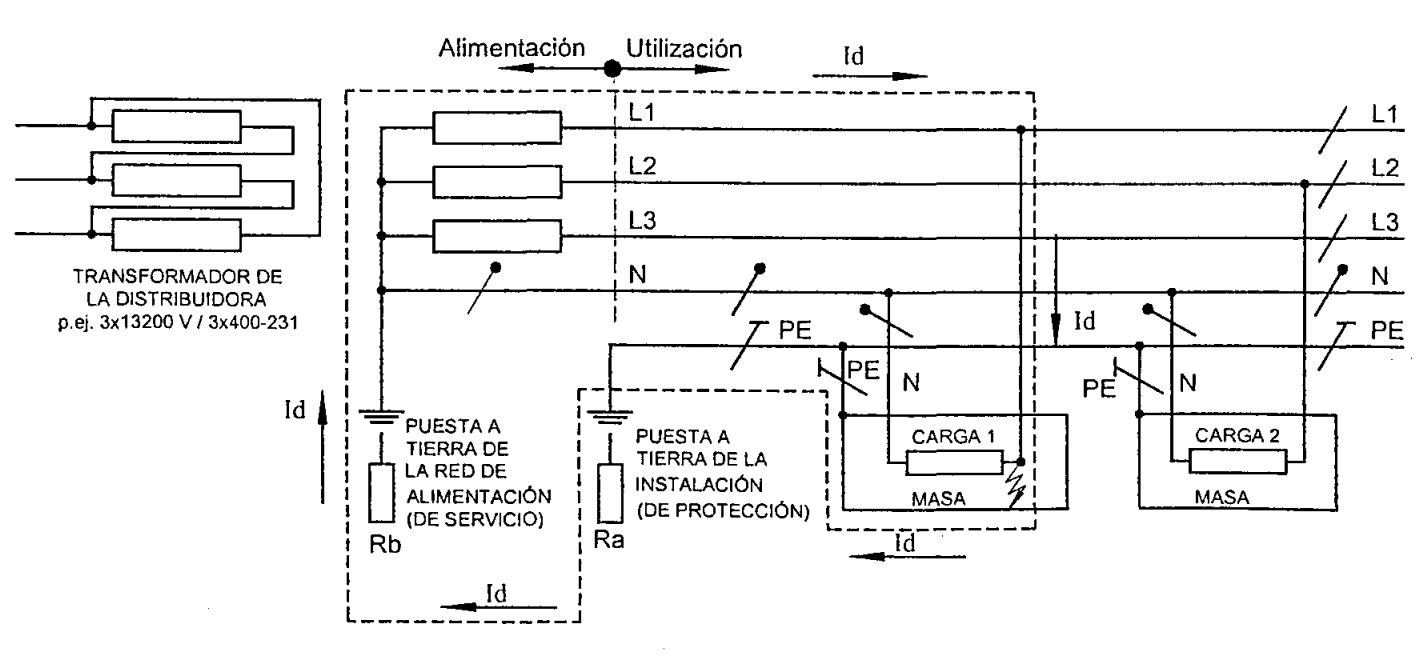
\includegraphics[width=\textwidth]{images/ect-tt}
  \caption{ECT TT. Fuente: AEA, 2006}
  \label{fig:ect-tt}
\end{figure}

En el esquema se puede apreciar la puesta a tierra de servicio $R_b$, la puesta a tierra de protección $R_a$, los conductores de puesta a tierra $PE$ conectados desde el electrodo $R_a$ a la \textbf{barra de puesta a tierra $PE$}, y a todos los tomacorrientes de tres espigas.
Al producirse un contacto indirecto, la corriente de defecto $I_d$ circulará desde la fase $L_1$ hasta el electrodo $R_a$, para luego recorrer por tierra la distancia que sea necesaria hasta alcanzar el electrodo de puesta a tierra de servicio $R_b$ y cerrar el circuito.

El valor de resistencia de puesta a tierra puede, según el reglamento, alcanzar los $40\; \Omega$ siempre y cuando la protección diferencial posea una corriente de disparo máxima de $300\; mA$.

Antiguamente se buscaba un valor menor a $10\; \Omega$ para la puesta a tierra, pero en realidad, esto era conveniente cuando no existía protección diferencial, debido a que esto haría que la corriente de falla sea mucho mayor, y activaría los termomagnéticos o fundiría los fusibles. Para sistemas con protección diferencial (como es obligatorio para el sistema TT), no es necesario que el valor óhmico de la puesta a tierra sea tan elevado.

\begin{ejemplo}
	Dada una puesta a tierra en un buen suelo, en el que se ha alcanzado una resistencia de puesta a tierra de $10\; \Omega$, y la distribuidora de energía posee una resistencia de puesta de servicio de $1\; \Omega$, la corriente de defecto se podría calcular según la Ley de Ohm, de la siguiente forma:
	
	$$I_d= \frac{V_{\text{línea}}}{\text{Suma de resistencias}}$$
	$$I_d = \frac{220\; V}{10\; \Omega + 1\; \Omega}=20\; A $$

	Es decir que ante una falla en una instalación típica, un valor de corriente cercano a $20\; A$ circulará por la rama de la corriente de defecto. Este valor es muy superior a los valores de corte de los interruptores diferenciales.
\end{ejemplo}

Las siglas TT indican Tierra-Tierra. Esto significa que el sistema dispone de una puesta a tierra de servicio y una puesta a tierra para la instalación por separado. La puesta a tierra de servicio es responsabilidad de la empresa distribuidora, mientras que la tierra de la instalación es trabajo del instalador.

Nunca se debe, en un esquema TT, conectar la tierra con neutro, debido a que la seguridad dependería de la calidad del neutro que entregue la compañía. Además, esto provocaría que el esquema se convierta en TN-S.

La Ley fija que la tensión de contacto máxima es de $24\; V$, y toda tensión superior en masas eléctricas o extrañas, deberá ser detectada por el diferencial e interrumpida de inmediato para evitar accidentes.

El protocolo exige medir $R_a$ (el cual deberá ser menor a $40\; \Omega$, verificar la continuidad de los conductores de protección (aquellos que van desde cada dispositivo y tomacorriente de tres contactos al conductor de tierra) y del conductor de tierra (que es el conductor que va desde el electrodo $R_a$ hasta la barra de puesta a tierra en el tablero principal. Se deberá verificar también, mediante los distintos ensayos, el dispositivo de protección que proteja contra contactos indirectos (interruptor diferencial). 

TN-S
%Imagen

Las instalaciones que utilizan este esquema son aquellos que toman en media tensión (como por ejemplo grandes industrias) o aquellos que han incorporado un transformador en su instalación, con el fin de adecuar el sistema a TN-S (por venir de un ECT TT).

Aquí el conductor de protección de la instalación se conecta a la barra de neutro. De ahí el nombre TN (Tierra-Neutro).

Por otra parte, se debe destacar que la conexión entre tierra y neutro se hace en las barras del tablero principal, pero los conductores de tierra y de neutro deberán estar separados a lo largo de la instalación (por ello la letra S en TN-S).

La corriente de falla se produce por los elementos metálicos (no por la tierra) y por ello es de muy alto valor y se permite utilizar fusibles o interruptores automáticos (además de diferenciales, como era el caso del esquema TT).

Dicho de otra forma, la resistencia $R_b$ no participa del lazo de corriente de falla, pero aún así debe poseer un valor muy bajo por otras razones: ... ESCRIBIR RAZONES


TN-C
Esquema.
Tiene tres problemas.
IT
Esquema.
Sólo en quirófanos.